\documentclass[a4paper,12pt]{scrartcl}

% usepackage definitions for KiekerTutorial.tex and for roadmap.tex
\usepackage{hyperref}
\newcommand{\goodgap}{\hspace{\subfigtopskip}\hspace{\subfigbottomskip}}
\usepackage{times}
\usepackage[latin1]{inputenc}
\usepackage{graphicx}
\usepackage{subfigure}
\usepackage{natbib}
\usepackage{listings}
\listfiles \lstloadlanguages{java} 
\lstset{language=java,
  showspaces=false,
  escapeinside={/*@}{@*/},
  showstringspaces=false,
  numbers=left,
  numberstyle=\tiny,
  numbersep=5pt,
  breaklines=true,
  breakautoindent=true,
  float=hbp,
  basicstyle=\ttfamily\small,
  columns=flexible,
  tabsize=2,
  extendedchars=true,
  frame=trbl
}
\newcommand{\todobox}[1]{\marginpar{\footnotesize \textbf{ TODO:  #1 }}}
\newcommand{\structurebox}[1]{%
	\par\noindent%
        \begin{center}
        \doublebox{\parbox{.8\columnwidth}{\texttt{Structure guide:} #1}}%
        \end{center}
}
\newcommand{\tpmon}{\textit{Tpmon}}
\newcommand{\tpan}{\textit{Tpan}}
\newcommand{\kieker}{\textit{Kieker}}
\newcommand{\tpmonltw}{\textit{tpmonltw.jar}}
\newcommand{\aspectjweaverjar}{\textit{aspectjweaver.jar}}



\newcommand{\kiekerurl}[1]{\small\url{http://www.matthias-rohr.com/kieker/#1}\normalsize}
\newcommand{\kiekertutorialurl}{\kiekerurl{KiekerTutorial.pdf}}
\newcommand{\kiekerroadmapurl}{\kiekerurl{KiekerTutorial.pdf}}

\title{Tutorial for \kieker : Monitoring and Visualization of Software Behavior \\ \small \vspace{3mm} DocumentURL: \kiekertutorialurl}
\author{The Kieker project \\ Matthias Rohr, Andr\'{e} van Hoorn, Nina Marwede}

\begin{document}
\maketitle
\tableofcontents
\section{Overview}

\todobox{
 Die alten Properies zum Einschalten von asynchr. FS bzw. DB sind weg!}

Kieker is a framework for monitoring the runtime behavior of Java software applications. It can be used for plain Java applications, or for Java Web-applications running in application servers. The resulting monitoring data can be converted to architectural models. 

\

Kieker aims to provide a maintainable monitoring solution for continuous application during normal operation in Java Web applications. Therefore, a major focus was on optimizing the monitoring overhead (not more than several milliseconds p. monitoring point invocation).

\

Since 2005, \tpmon{} was used by several industry partners in portal systems and enterprise information systems during regular operations. Additionally, it is regularly used in the laboratory for research on software timing behavior and timing behavior anomaly detection at the University of Oldenburg, University of Kiel. Since August 2008, \tpmon{} is a sourceforge project.

\

Besides monitoring, Kieker will allow\footnote{Not included in this release; ask for prototypes, if desired.} to create and visualizes models of current or past software system behavior in terms of \textbf{UML Sequence Diagrams}, \textbf{Markov chains} (for user requests or user sessions), \textbf{Component Dependency Graphs}, \textbf{Dynamic Call Trees}~\citep{AmmonsBallLarus97ExploitingHardwarePerformanceCountersWithFlowAndContextSensitiveProfiling}, Trace Timing Diagrams, as well as Execution and Message trace models. Figure~\ref{visualizationExample1} shows an UML Sequence Diagram and a Dynamic Call Tree based on visualizations generated by Kieker.

\

Kieker consists of two major components: the monitoring component \textbf{\tpmon}\ and the analysis and visualization component \textbf{\tpan}. \tpan{} may be part of a future release; don't hesitate to contact us for our research prototype of \tpan{}. Both operate rather independently and are connected by a simple monitoring data format. %This allows one to analyze data from an other monitoring tool with \tpan\ and to use \tpmon's  monitoring data in other tools with only shell based modifications.

\begin{figure}
\centering
\subfigure[UML Sequence Diagram.]{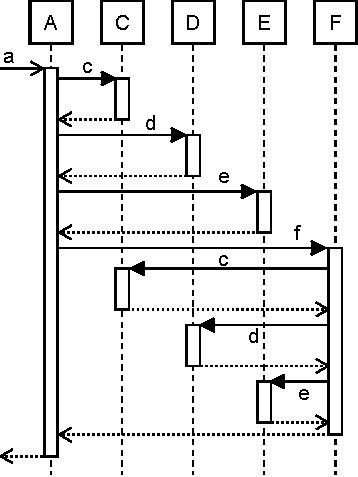
\includegraphics[width=4.3cm]{seqDia2-small.pdf}}
\hspace{1cm}
\subfigure[Dynamic call tree.]{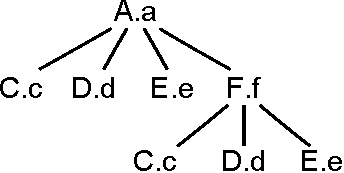
\includegraphics[width=4.5cm]{dct-2-small.pdf}}
\caption{UML Sequence Diagram and its corresponding Dynamic Call Tree~\citep{RohrVanHoornGieseckeMatevskaHasselbring08TraceContextSensitivePerformanceModelsFromMonitoringDataOfSoftwareSystems}.
}\label{visualizationExample1}
\end{figure}

\

Kieker focuses on monitoring method (or service) calls. Therefore, it can be called a \textit{service-level} monitoring tool or \textit{application-level} monitoring tool. If monitoring of single statements (e.g., \small \texttt{a = a + 1}\normalsize) is required other profiling tools such as Intel's VTune should be used. Keep in mind that these tools, which can be denoted \textit{statement-level monitoring} (= algorithm-level), usually are much more resource demanding and not supposed for continuous operation in production systems, because of the finer monitoring granularity.

\subsection{Monitoring using \tpmon}

\tpmon\ is the instrumentation and monitoring component of \kieker. It integrates monitoring points into Java programs using aspect-oriented programming (AOP), records response times and calling paths, and stores the monitoring data into the local file system or into a database management system, such as MySQL. 

\

Four steps are required to instrument a Java software application with \tpmon:
\begin{enumerate}
\item Download of \tpmon\ from \kiekerurl{}
\item Configuration of \tpmon{}  (e.g., storage in file system or in a database)
\item Specification of monitoring points 
\item Integration of monitoring code: Adaptation of the build- or startup-scripts of the application to be monitored; 
\end{enumerate}

A quick tutorial for instrumenting software with \tpmon{} is provided in Section~\ref{sec.tpmon.tutorial}.

\subsubsection{Manual instrumentation}
In the following, we demonstrate manual usage (manual instrumentation) for monitoring using \tpmon{}. It has to be mentioned, that manual instrumentation is not using one of \tpmon's major features - the automatic monitoring code integration mechanism. However, for demonstration purposes, a manual usage of the \tpmon-framework is shown in Listing~\ref{manualInstrumentation}. The suggested, less intrusive, and more maintainable solution is presented in Listing~\ref{placingAnnotation} of Section~\ref{sec.tpmon.tutorial}. The manual  instrumentation consists of recording two timestamps (Line 8 and 12) and an invocation of \tpmon{}'s data management mechanism (Line 13). On executing the program, a monitoring observation will be stored by default in the file system.

\begin{lstlisting}[caption={\footnotesize\texttt{src/kieker/tests/helloWorld/manualInstrumentation/HelloWorld.java}},label={manualInstrumentation}]
package kieker.tests.helloWorld.manualInstrumentation;
import kieker.tpmon.TpmonController;
public class HelloWorld {
    public static void main(String args[]) {
        System.out.println("Hello");
        
        /* recording of the start time of doSomething */
        long startTime = System.nanoTime();
        
        doSomething();
        
        long endTime = System.nanoTime();
        TpmonController.getInstance().insertMonitoringDataNow("kieker.tests.helloWorld.manualInstrumentation.HelloWorld", "doSomething()", "request1", startTime, endTime);
                
        /* System.exit() called to initiate shutdown of 
         * the monitoring logic running in seperate threads */
        System.exit(0);
    }

    static void doSomething() {
        System.out.println("doing something");
        /* .. some application logic does something meaningful ..*/        
    }
}
\end{lstlisting}

\subsection{Analysis and Visualization using \tpan}
A research prototype of \tpan\ is available on demand\footnote{Email to: rohr(a-t)informatik.uni-oldenburg.de, van.hoorn(a-t)informatik.uni-oldenburg.de.}. A step-wise release of \tpan{} is planed for Q1 2009.

\subsection{Document Structure}

Section~\ref{sec.tpmon.tutorial} contains a small tutorial for \tpmon while the manual \tpmon\ is in Section~\ref{sec.tpmon}.% and \ref{sec.tpan}. %Section~\ref{} presents some empirical results that characterize the monitoring overhead of \tpmon.



\section{\tpmon\ Quick Start Guide -- Hello World}\label{sec.tpmon.tutorial}
In the following, the steps to instrument a Java program with \tpmon\ are briefly explained and demonstrated in the context of a Hello World example. Kieker's alternative monitoring and instrumentation modes are explained in detail in Section~\ref{sec.tpmon}.

\

\tpmon's essential \textbf{system requirements} are that at least Sun's Java SE 5 (JDK) (Version number $\geq$ 1.5.0) and Apache Ant\footnote{Available at \url{http://ant.apache.org/}} 1.7 are installed. \tpmon\ has been tested on Linux, Solaris, FreeBSD and Windows.

\subsection{Downloading Kieker}
The first step is to download the latest Kieker release from \kiekerurl{} and to decompress it into a folder of your choice. This folder is denoted \texttt{\$KIEKERHOME} in the remainder of this document. You may set it as environment variable\footnote{The error message ``Error opening zip file or JAR manifest missing : /external-libs/aspectjweaver.jar'' means that you used this environment variable without having it set correctly.}, so that you can directly execute the commands shown in this Section.
\begin{itemize}
 \item Linux/Unix: e.g., % KIEKERHOME=/home/matthias/projekte/kieker/sourceforge/kieker/
\begin{lstlisting}[caption={}] 
KIEKERHOME=/home/matthias/sourceforge/kieker
\end{lstlisting}
\item Windows: e.g.,
\begin{lstlisting}[caption={}]
set KIEKERHOME=c:\sourceforge\kieker
\end{lstlisting}
\end{itemize}

\subsection{Configuration of \tpmon}
The major configuration file for the monitoring is \texttt{\$KIEKERHOME}$\backslash$\texttt{tpmon.properties}. It specifies properties such as the folder for storing monitoring data and allows to select different storage modes (e.g., database or file system). The \texttt{tpmon.properties} must be created from \texttt{tpmon.properties.example}, if it doesn't exist. There are two ways to configure the data storage directory: 
\begin{enumerate}
\item (Default) Store into the system's default temporary folder (java.io.tmpdir). For UNIX systems this is often \texttt{/tmp} and on Microsoft Windows systems it is typically some folder like \verb=C:\\Docum...\USER...\Temp=. Be aware that the temporary folders may be deleted each time automatically by the operation system, e.g., after system restart. If the monitoring is used in an application server, \textit{java.io.tmpdir} might be defined differently. 
\item Store monitoring data into an explicitly specified folder.
\end{enumerate}
These modes can be configured via the \texttt{tpmon.properties} file via the properties \textit{tpmon.storeInJavaIoTmpdir} and \textit{tpmon.customStoragePath}. Additionally, it is possible to overwrite these and several other properties file settings via the Java command line parameters \footnotesize \texttt{java -Dtpmon.storeInJavaIoTmpdir=false -Dtpmon.customStoragePath=/var/log/}. \normalsize

An example for the settings in the \texttt{tpmon.properties} file are given in the following listing:
\begin{lstlisting}[caption={Linux/Unix: Specification of the monitoring data storage location}]
...
#1.3.1.a (should the systems default temporary folder by used?)
tpmon.storeInJavaIoTmpdir=true

#1.3.1.b (use this custom storage folder)
# e.g., /var/tpmon/ or "c:\tmponData\" (ensure the folder exists)
tpmon.customStoragePath=/tmp/
...
\end{lstlisting}

The other settings do require changes for this example. The default settings are that \tpmon\ stores monitoring data in the file system using an asynchronous file system writer into the system's default temporary folder.

\subsection{Building the \tpmon{} library}

\tpmon\ has to be recompiled to activate any changes in the properties file and to create the monitoring library\footnote{\texttt{KiekerTpmonCtrl-VERSION.jar}} required during runtime:
\begin{lstlisting}[]
ant build-all
\end{lstlisting}
This produces three new files \texttt{\$KIEKERHOME}/\texttt{dist}/\texttt{KiekerTpmonCTW-0.VERSION.jar} for compile-time instrumentation, \texttt{KiekerTpmonLTW-VERSION.jar} for load-time instrumentation, and the stand alone library \texttt{KiekerTpmonCtrl-VERSION.jar} that can be used by other instrumentation frameworks to organize tracing and data storage, e.g., within an application server.

\subsection{Specification of monitoring points}\label{sec.tutorial.annotation}
Next, the following program \texttt{HelloWorld.java} will be instrumented. The source code can be found in the folder \textit{src/kieker/tests/helloWorld}.
\begin{lstlisting}[caption={\texttt{HelloWorld.java}},label={lst1}]
public class HelloWorld {	
	public static void main (String args[]) {
		System.out.println("Hello");
		doSomething();
	}
	public static void doSomething(){
		System.out.println("doing something");
	}
}
\end{lstlisting}

In this example, Java Annotations are used to specify the Java methods to be monitored. In Listing~\ref{placingAnnotation} it is illustrated how to instrument the two Java methods \texttt{main} and \texttt{doSomething} by the Java Annotations in Line~3 and 9. These annotations trigger the aspect-oriented programming tool AspectJ to integrate monitoring logic into the application during runtime or during compile time. The \texttt{import} in Line~1 is required to define the Annotation.

\begin{lstlisting}[caption={Lines 1, 3 and 9 are added to instrument this simple ``Hello World'' Java program.},label={placingAnnotation}]
import kieker.tpmon.annotations.TpmonMonitoringProbe;
public class HelloWorld {
	@TpmonMonitoringProbe()
	public static void main (String args[]) {
		System.out.println("Hello");
		doSomething();
	}
	
	@TpmonMonitoringProbe()
	public static void doSomething(){
		System.out.println("doing something");
	}
}
\end{lstlisting}

\subsection{Integrating Monitoring Code}
\tpmon\ supports the integration of monitoring logic at the time of compilation (of the application to be monitored) or during runtime (= at class load-time). In this example, load-time integration of monitoring code into the application to be monitored will be used. This requires the execution of the following two commands:

\begin{lstlisting}[caption={Compilation and execution with AspectJ's Java agent.},label={javaHelloWorld}]
javac -cp $KIEKERHOME/dist/KiekerTpmonCtrl-0.91.jar HelloWorld.java
java  -javaagent:$KIEKERHOME/external-libs/aspectjweaver.jar -cp $KIEKERHOME/dist/KiekerTpmonLTW.jar:.:  HelloWorld
\end{lstlisting}
If the first command does not compile, the \tpmon{} library is not found\footnote{Error message: cannot find symbol @TpmonMonitoringProbe} in the classpath or the import statement contains a typo. 

\

Listing~\ref{javaHelloWorld} should result in output like shown in Listing~\ref{OutputHelloWorld}.
\begin{lstlisting}[caption={Compilation and execution with AspectJ's Java agent.},label={OutputHelloWorld}]
Hello
doing something
 The vmid is 9069ca78e7450a28:5996e72a:119c2f563bd:-7fff hashcode -1024138306
 Virtual Machine start time 1210156670849
Tpmon: TpmonShutdownHook notifies all workers to initiate shutdown
Tpmon: TpmonShutdownHook can terminate since all workers are finished
\end{lstlisting}
Lines~1 and 2 are produced by the \texttt{println}s of \texttt{HelloWorld}. The other lines are \tpmon\ status information.

\

Note, the command \texttt{java  HelloWorld} does not fail if  \tpmon\ is not in the classpath. Weaving and integration of monitoring logic is only performed if both the AspectJ javaagent is loaded into the Java VM \textit{and} the \tpmon\ load-time library is in the classpath.

\paragraph{More verbose output}
Additional verbose output, such as on which Java files are woven, is produced for:
\begin{lstlisting}[caption={Verbose execution with AspectJ's Java agent.},label={lst2}]
java -Daj.weaving.verbose=true -Dorg.aspectj.weaver.showWeaveInfo=true -javaagent:$KIEKERHOME/external-libs/aspectjweaver.jar -cp $KIEKERHOME/dist/KiekerTpmonLTW.jar:.:  HelloWorld

info AspectJ Weaver Version 1.5.2a built on Friday Aug 18, 2006 at 18:40:31 GMT
info register classloader sun.misc.Launcher$AppClassLoader@32582734
info using configuration file:/home/matthias/projekte/kieker/sourceforge/kieker/dist/KiekerTpmonLTW.jar!/META-INF/aop.xml
info register aspect kieker.tpmon.aspects.TpmonMonitorAnnotation
info weaving 'HelloWorld'
...
\end{lstlisting}
Line~7 provides the important status information that \tpmon's monitoring code is woven into HelloWorld.



\paragraph{Monitoring data}
The monitoring data for Listing~\ref{javaHelloWorld} is written to a file which is named \texttt{/tmp/tpmon--*-*.dat}, where $*$ represents some number. It should contain two lines like:
\begin{lstlisting}[caption={Example monitoring data},label={OutputHelloWorld2}]
0;HelloWorld.doSomething();nosession;1210156671935-1-0; 1210156671935804069;1210156671940322555;-1024138307;-1;-1
0;HelloWorld.main(java.lang.String[]);nosession;1210156671935-1-0; 1210156671935203951;1210156671948286691;-1024138307;-1;-1
\end{lstlisting}

Columns~5 and 6 are start timestamps and end timestamps for executions of operations. The timestamps are provided in nanoseconds since 1.1.1970. The monitoring data file is a CSV file. Instead of commas, it uses semi-colons as separators, because commas can be part of operation names (e.g., \texttt{sum(int a,int b)}). A detailed description of the monitoring data format can be found in Section~\ref{sec.monitoring.data.format}.

\section{\textit{Tpmon}: Instrumenting and Monitoring Java Applications}\label{sec.tpmon}

The small tutorial in Section~\ref{sec.tpmon.tutorial} uses only one of \tpmon's monitoring modes. You have to make the following design decisions when you are using \tpmon:
\begin{itemize}
 \item When and how should the monitoring logic be integrated?
\begin{itemize}
 \item \textbf{Compile-time integration} (using compile-time-weaving): In this mode, you the build-scripts or build-commands of your Java program are adjusted, such that the bytecode is already instrumented. During runtime, no aspect-oriented programming features (related to reflection and class loading) are required and only the \tpmon library has to be added to the execution classpath.
\item Class \textbf{load-time integration}: Load-time integration combines monitoring logic with program logic of a class at the time the Java Virtual Machine accesses program class for the first time (during runtime. A advantage of load-time weaving is that no large changes to the build scripts are required (only \tpmon\ might have to be added to the compile-time classpath). It is can also be used to instrument (full instrumentation) programs for that no source code is available. However, the start-scripts for your application, or the configuration files of the middleware that runs your application, have to be extended by adding the AspectJ javaagent that combines monitoring logic and program logic during runtime. Load-time integration may fail in some environments that use special dynamic features such as reflection, customized class-loaders, and particular types of remote communication. For instance, runtime instrumentation fails for Eclipse Plugins\footnote{Other profilers have also problems with profiling Eclipse Plugins}, RMI objects (code base changes are detected and cause exceptions), and for classes and objects that are defined during runtime via reflection, such as it is used for the Hessian Web-service library.
\end{itemize}
\item Which Java methods should be monitored?
\begin{itemize}
\item \textbf{Full instrumentation}: A full instrumentation of a complete Java package does not require changes of the source code of the program to be monitored. However, instrumenting all methods within a package can impose a too large monitoring overhead. 
\item \textbf{Partial instrumentation}: Partial instrumentation is done by placing a special Java Annotation in front of every Java method for which instrumentation is desired. The annotations can be used by compile-time integration or load-time integration. 
\end{itemize}
\item Where should the monitoring data be stored?
\begin{itemize}
\item \textbf{File system}: Storing the monitoring data into the file system is the most performant data storage mode of Kieker. However, if the files have to be transported regularly to an other host for analysis, it might be better directly store it into a remote database. In particular if continuous monitoring during regular operation is required, it is suggested to transfer the monitoring data just after it has been observed to an other host's database for persistent storage and analysis.
\item \textbf{Database management system}: Database management systems provide means to efficiently store large amounts of data and provide a powerful query language for data access. \tpmon\ requires a small additional overhead for storing in a remote database system compared to storing in a local file system. The overhead (e.g., 0.1-5 milliseconds in average) is only a problem if precise timing analysis, e.g., for anomaly detection, is required. %However, this overhead does occur anyhow if the monitoring data has to be analyzed on a remote platform. 
\end{itemize}
\end{itemize}

\subsection{Downloading Kieker}
The latest Kieker release can be downloaded from \kiekerurl. The folder where the uncompressed release is located on your hard disc is denoted \texttt{\$KIEKERHOME} in the remainder of this document. You may set it as environment variable, so that you can directly execute the commands shown in this section
\begin{itemize}
 \item Linux/Unix: e.g.,
\begin{lstlisting}[caption={}]
KIEKERHOME=/home/matthias/sourceforge/kieker
\end{lstlisting}
\item Windows: e.g.,
\begin{lstlisting}[caption={}]
set KIEKERHOME=c:\sourceforge\kieker
\end{lstlisting}
\end{itemize}

\subsection{\tpmon's configuration file \texttt{tpmon.properties}}\label{sec.tpmon.properties}

\todobox{
 Der MonitoringWriter l�sst sich nun �ber ein Property einschalten:
    monitoringDataWriter=SyncFS|AsyncFS|SyncDB|AsyncDB
    (nat�rlich nur eine dieser Konstanten)
    �ber dieses Property lassen sich nun auch Writer per Namen laden,
    z.B.
monitoringDataWriter=src.kieker.tpmon.extra.asyncJmsWriter.AsyncJmsProducer
    Diese Writer lassen sich �ber die Property
    monitoringDataWriterInitString konfiguieren. Im JMS-Beispiel:
    monitoringDataWriterInitString =
jmsProviderUrl=tcp://localhost:3035/ | jmsTopic=queue1 |
jmsContextFactoryType=org.exolab.jms.jndi.InitialContextFactory |
jmsFactoryLookupName=ConnectionFactory | jmsMessageTimeToLive = 10000
}

\todobox{
 Die alten Properies zum Einschalten von asynchr. FS bzw. DB sind weg!}



The configuration file \texttt{tpmon.properties} specifies \tpmon's runtime behavior (database or file system 
storage) and the path to required libraries for the build process. In the following, we explain properties (default settings are underlined):

\begin{description}
 \item [1.1.1] \texttt{storeInDatabase=[true$|$\underline{false}]} \\
Here it is specified whether \tpmon\ stores the data in a remote database or in the local file system. 
\item [1.1.2] \texttt{debug=[true$|$\underline{false}]}  \\
In debug mode, tpmon is very verbose during runtime.
\item [1.1.3] \texttt{monitoringEnabled=[\underline{true}$|$false]} \\
Should monitoring be enabled right after the application start? You can also use the tpmon-control-servlet
to activate monitoring later.
\item [1.2.1] \texttt{dbconnectionAddress=} \\
Specifies the database connection parameter for the initialization of the database connection. Example: 
\small
\texttt{jdbc:mysql://HOST/DATABASENAME?user=USER\&password=PASS}
\normalsize
\item [1.2.2] \texttt{dbTableName=\underline{turbomon9}} \\
Name of the database table. The SQL statement for creating a suitable database table
in MySQL can be found in file \small \texttt{table-for-monitoring.sql}\normalsize.
\item [1.2.3] \texttt{setInitialExperimentIdBasedOnLastId=[true$|$\underline{false}]} \\
Should \tpmon\ look into the database for the last experiment identifier and use a new one increased by one?
\item [1.2.3] \texttt{useAsyncDbconnector=[\underline{true}$|$false]} \\
If true, \tpmon\ uses a connection pool for storing data into the database. This is more performant and the communication
with the database runs in separate threads so that the application under monitoring has not to wait each time a monitoring
observation has to be stored.
\item [1.3.1] \footnotesize \texttt{tpmon.storeInJavaIoTmpdir=[\underline{true}$|$false]} $\&$ \texttt{tpmon.customStoragePath=..} \normalsize \\ 
There are two ways to specify where \tpmon\ should place its monitoring data files (\texttt{tpmon-*-*.dat}).: 
\begin{enumerate}
\item [a] \texttt{tpmon.storeInJavaIoTmpdir=[\underline{true}$|$false]} \\ Store into the system's default temporary folder (java.io.tmpdir). For UNIX systems this is often defaults to \texttt{/tmp} and on Windows systems to some folder like \verb=C:\Docum...\USER...\Temp=. Be aware that the temporary folders may be deleted each time automatically by the operation system, e.g., after system restart.
\item [b] \texttt{tpmon.customStoragePath=/tmp/} \\ Store monitoring data into an explicitly specified folder.
\end{enumerate}
These modes can be configured via the \texttt{tpmon.properties} file. Additionally, it is possible to overwrite the properties file setting via the Java command line parameters \footnotesize \texttt{java -Dtpmon.storeInJavaIoTmpdir=false -Dtpmon.customStoragePath=/var/log/}. \normalsize 

A new file will be created each 22,000 lines.

An example for the settings in the \texttt{tpmon.properties} file are given in the following listing:
\begin{lstlisting}[caption={Linux/Unix: Specification of the monitoring data storage location}]
...
#1.3.1.a (should the systems default temporary folder by used?)
tpmon.storeInJavaIoTmpdir=true

#1.3.1.b (use this custom storage folder)
# e.g., /var/tpmon/ or "c:\tmponData\" (ensure the folder exists)
tpmon.customStoragePath=/tmp/
...
\end{lstlisting}

\item [1.3.2] \texttt{asyncFsWriter=[true$|$\underline{false}]} \\ 
If true, \tpmon\ will use a pool of independent threads to store monitoring data in the file system. This results in less outliers in the monitoring data that can occur for I/O processing. You can safely use \texttt{true} here, but you will have to add a \texttt{system.exit(0)} to your application (not required for application servers, or servlet containers) or it will never terminate. \tpmon\ ensures that no data is lost when the application terminates normally.
\item [2.1] \texttt{tpmon.javac.debug=[true$|$\texttt{false}]} \\
If true, \texttt{javac} will be called with the debug flag. 
\end{description}

\subsection{Building the \tpmon\ Libraries}
The \tpmon\ libraries (\texttt{KiekerTpmonLTW.jar} and \texttt{KiekerTpmonCTW.jar}) have to be recompiled each time \texttt{tpmon.properties} or \texttt{aop.xml} is changed. The command for rebuilding \tpmon\ is \texttt{ant build}. If compilation succeeds, Ant returns \texttt{BUILD SUCCESSFUL} and the two libraries are created in the folder \texttt{dist}.

By default, the \tpmonltw\ will be configured to look for potential monitoring points in all packages except in the Java's own libraries and in some internal Kieker packages. %To monitor your own software application you have to set monitoring points as described in Section~\ref{settingOfMonitoringPoints}. 

% \subsection{Testing  \tpmonltw}
% %After building an \tpmonltw its a good idea to test whether the monitoring works for Kieker's small example application. Before Kieker is used to monitor your own application.
% By default, Kieker will only instrument Java methods that have the source code instrumentation \texttt{@TpmonMonitoringProbe()} (see Example~\ref{}). Additionally, \tpmon is configured to only look for monitoring points in the Java package \texttt{kieker.tests ..*}.
% The monitoring data will be stored in the file system to the folder \texttt{$\$tmp$\$ } having names \texttt{tpmon-*.dat}, where \texttt{*} is some number based on the timestamp of file creation.
% 
% 
% % \subsection{Setting Monitoring Points}\label{settingOfMonitoringPoints}

\subsection{Instrumentation}
As discussed at the beginning of this section, you have to chose
 whether you want that the monitoring logic is combined with the application
 logic during during load-time, i.e., the time at which the Java Virtual Machine
 load class file when they are required the first time during runtime, or at compile-time. Additionally,
you have to chose whether full or partial instrumentation should be used.

% \
% 
% Load-time instrumentation requires that the run-scripts
% of the application, or of the hosting middleware have to be adjusted. Additionally, some special 
% Java runtime features (e.g., reflection API) will be used that might cause problems in some cases.
% 
\subsubsection{Load-time instrumentation}
There are two possible modes for load-time instrumentation supported by \tpmon:
 Full instrumentation of selected Java packages and partial instrumentation via Java Annotations
in the program source code.
\paragraph{Full instrumentation}
This variant, i.e. full instrumentation via load-time weaving, can be used if no source code is available. This means only the \texttt{.jar} or \texttt{.class} files have to be provided. However, all methods of the classes in the packages specified in the \texttt{aop.xml} are monitored by the aspect \texttt{TpmonMonitorFullInstrumentation}, which may cause large monitoring overhead.

\begin{itemize}
 \item Specification of packages to instrument in \texttt{aop.xml}\footnote{Located in \texttt{src/kieker/tpmon/META-INF/}}: Specify in the first part of the \texttt{aop.xml} via \texttt{include} \texttt{exclude} tags which packages should be instrumented. Take a look at  \texttt{aop.xml.example} for examples.
\item Activating the full-instrumentation aspect in \texttt{aop.xml}: In the last part of the \texttt{aop.xml} uncomment the aspect \texttt{TpmonMonitorFullInstrumentation} and put all other aspects into comments.
\end{itemize}

Full instrumentation via load time weaving can be tested using the ant build target \\ \small \texttt{run-tests-loadTimeWeaving-bookstoreWithoutAnnotation} \normalsize of the \texttt{build.xml} tpmon package. For this test, only the \texttt{aop.xml} needs to be adjusted, as described above.

\paragraph{Partial instrumentation (using Java Annotations)}
\begin{itemize}
 \item Specification of packages to instrument in \texttt{aop.xml}\footnote{Located in \texttt{src/kieker/tpmon/META-INF/}}: Specify in the first part of the \texttt{aop.xml} via \texttt{include} \texttt{exclude} tags which packages will be scanned for the \texttt{TpmonMonitoringProbe} Java Annotations. Take a look at  \texttt{aop.xml.example} for examples.
\item Specification of the instrumentation mode \texttt{aop.xml}: In the last part of the \texttt{aop.xml} uncomment the aspect \texttt{TpmonMonitorAnnotation} and put all other aspects into comments.
\item Modify the source code of the program to be instrumented such as in the Listing~\ref{placingAnnotation} of the Section~\ref{sec.tutorial.annotation}. Also add the \texttt{import} as in Line 1 of Listing~\ref{placingAnnotation}.
\end{itemize}

\subsubsection{Compile-time instrumentation}

For compile-time instrumentation, it is required install the AspectJ compiler from \url{http://www.eclipse.org/aspectj/}.

\paragraph{Full instrumentation}
\begin{itemize}
 \item Copy the aspect file \small \texttt{TpmonMonitorFullInstrumentation.aj}\normalsize\ into a folder of your program sources.
\item In your application build-scripts, replace the compiler with the AspectJ compiler. Add \texttt{KiekerTpmonCTW.jar} to compilation classpath. An example ant script target for this compilation can be found in \tpmon's \texttt{build.xml} (see target \\ \texttt{compile-tests-compileTimeWeaving-bookstore}).
\end{itemize}

\paragraph{Partial instrumentation (using Java Annotations)}
\begin{itemize}
\item  Copy the aspect file \small \texttt{TpmonMonitorAnnotation.aj}\normalsize\ into a folder of your program sources.
\item Modify the source code of the program to be instrumented as shown in Listing~\ref{placingAnnotation} of the Section~\ref{sec.tutorial.annotation}. Also add the \texttt{import} as in Line 1 of Listing~\ref{placingAnnotation}.
\item In your application build-scripts, replace the compiler with the AspectJ compiler. Add \texttt{KiekerTpmonCTW.jar} to the compilation classpath. An example ant script target for this compilation can be found in \tpmon's \texttt{build.xml} (see target \\ \texttt{compile-tests-compileTimeWeaving-bookstore}).
\end{itemize}


\subsection{Executing the instrumented program} 

The execution scripts and application server startup scripts have to be adjusted to run the instrumented program with monitoring. 

\paragraph{Executing compile-time instrumented programs}

Only the \texttt{KiekerTpmonCTW.jar} has to be added to the runtime classpath in order to execute programs that have been instrumented with compile-time instrumentation. It is also be required to the database driver to the classpath if database storage was selected. Output similar to that in Lines 6 and 7 in Listing~\ref{ExecutingCompileTimePrograms} results short after the first instrumented method is executed.

\begin{lstlisting}[caption={Execution of a compile-time instrumented program},label={ExecutingCompileTimePrograms}]
java  -cp $KIEKERHOME/dist/KiekerTpmonCTW.jar:.:  Main

...
The vmid is 9069ca78e7450a28:5996e72a:119c2f563bd:-7fff hashcode -1024138306
Virtual Machine start time 1210156670849
...
\end{lstlisting}

\paragraph{Executing load-time instrumented programs}

Executing load-time instrumented programs requires:
\begin{itemize}
\item adding \texttt{KiekerTpmonLTW.jar} to the runtime classpath (maybe also the database driver), and
\item adding the parameter \texttt{-javaagent:ADJUST/aspectjweaver.jar} to the Java Virtual Machine startup call.
\end{itemize}

To activate monitoring for load-time instrumented programs in the Apache Tomcat servlet container, add the following line to Tomcat's \texttt{catalina.sh} (right at the beginning of the file):
\begin{lstlisting}[caption={}]
JAVA_OPTS="-javaagent:ADJUST/aspectjweaver.jar"
\end{lstlisting}
Windows users have to add "set" in front of this line.

\

An example for executing a load-time instrumented program can be found in the tutorial in Section~\ref{sec.tpmon.tutorial}.

\subsection{Monitoring data format}\label{sec.monitoring.data.format}

\begin{figure}
 \centering
 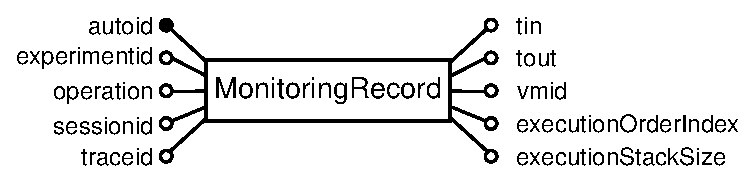
\includegraphics[width=0.8\columnwidth]{08-05-06-monitoringDataFormat}
 \caption{Database schema for the monitoring data (version 0.9).}
 \label{databaseSchema}
\end{figure}

The \textbf{database schema} of the monitoring data is displayed in the Entity-relationship Diagram (Figure~\ref{databaseSchema}). The data format for \textbf{monitoring data files} only differs to this schema by not containing the first column \texttt{autoid}. Each entry, called monitoring record, contains two timestamps (\texttt{tin} and \texttt{tout}) that denote the start time and end time of an operation execution, and attributes that describe a context of the measurement (\texttt{experimentid}, \texttt{operation}, \texttt{sessionid}, \texttt{traceid}, \texttt{vmid}). The \texttt{operation} attribute names the operation that corresponds to the execution monitored, and \texttt{traceid} is unique for executions of the same trace. %In a Java Web application, one user request (e.g., a single HTTP request) results in one or more traces.
 Java Web application technology provides the concept of sessions (monitored as \texttt{sessionid}) that connect single user requests. %Sessionid If available, ``sessionid'' is in a 1:m relation to ``traceid''. 
The \texttt{vmid} allows to distinguish different Java Virtual Machines. %Response times are the difference between the start and the 
The \texttt{executionOrderIndex} and \texttt{executionStackSize} are used if \tpmon\ monitors distributed systems. Local clock times are not a reliable source for determining the order of executions (e.g., for creating Sequence Diagrams) in a distributed system.

\begin{lstlisting}[caption={SQL script for preparing the database table},label={OutputHelloWorld3}]
 CREATE TABLE turbomon9 (
`autoid` BIGINT NOT NULL AUTO_INCREMENT PRIMARY KEY ,
`experimentid` SMALLINT NOT NULL DEFAULT '0',
`operation` VARCHAR( 160 ) NOT NULL ,
`sessionid` VARCHAR( 34 ) NOT NULL ,
`traceid` VARCHAR( 34 ) NULL ,
`tin` BIGINT( 19 ) UNSIGNED NOT NULL ,
`tout` BIGINT( 19 ) UNSIGNED NOT NULL ,
`vmid` INT( 10 ) NOT NULL DEFAULT '-1',
`executionOrderIndex` INT( 10 ) NOT NULL DEFAULT '-1',
`executionStackSize` INT( 10 ) NOT NULL DEFAULT '-1',
INDEX (operation(16)), INDEX (traceid), INDEX (tin)
) ENGINE = MYISAM;
\end{lstlisting}

\subsection{Monitoring overhead}

The monitoring overhead depends on many aspects such as the number of monitoring points, on the workload, and on the monitoring point invocation frequency. Therefore, it is no possible to specify the monitoring overhead in general. Since \tpmon\ is created for continuous operation during regular operation, it is designed to keep the monitoring 
overhead reasonably low. 

\textit{Tpmon} is installed in several production system of industry partners to instrument the most important services (about 50 monitoring points to say a number). No significantly noticeable monitoring overhead was reported for these installations. In general, it is our experience that imposing less than 10-20\% overhead on response times is accepted by enterprise system administrators in exchange for monitoring and its benefits. 

In the case studies using our instrumentation prototype Kieker, we observed an overhead on response times of 14\% for the default asynchronous file system storage mode (TpmonAsyncFs) (see Section~\ref{sec.tpmon.properties}). To quantify the overhead, a case study was performed using the iBATIS JPetStore demo Web-application. This software was deployed in a standard Java servlet container (Apache Tomcat). Probabilistic medium-level multi-user workload was generated using Markov4JMeter and Apache JMeter. Based on Tomcat's access logs (12 services for JPetStore) we compared container measured response times without and with \tpmon\ monitoring using 19 \tpmon\ monitoring points.

In Figure~\ref{MonitoringOverhead2} and Table~\ref{generatedTpmonPerfTabel} and  \ref{generatedTpmonPerfTabel2} the response time statistics of various instrumentation variants in the case study are compared. Table~\ref{generatedTpmonPerfTabel} shows that the asynchronous writing to the local file system is the most performant storage mode, imposing in average an overhead of 14\%. These results conform with the results provided by \citet{GovindrajNarayananThomasNairP06OnUsingAOPforApplicationPerformanceManagement} reporting about 10\% overhead for the 
monitoring framework InfraRED, which also uses aspect-oriented programming (AOP).

For distributed software systems, an additional overhead exists for remote communication, in order to connect traces over multiple nodes. 




% out of date -- less outliers are produced now
% \begin{figure}
%  \centering
%  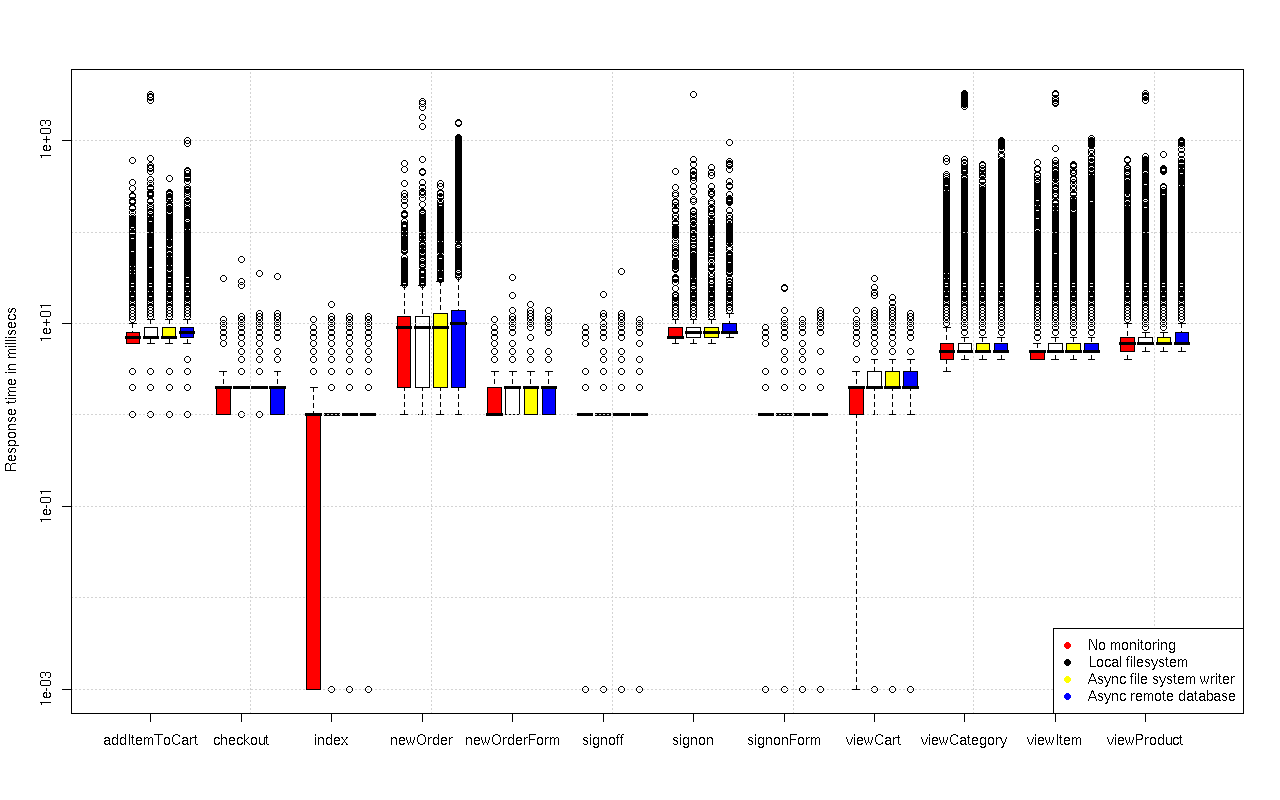
\includegraphics[width=\textwidth]{MonitoringOverhead0.png}
%  % MonitoringOverhead2.png: 1280x800 pixel, 72dpi, 45.16x28.22 cm, bb=0 0 1280 800
%  \label{MonitoringOverhead0}
%  \caption{JPetStore: Comparison of Monitoring Overhead (Logarithmic scale)}
% \end{figure}
% \begin{figure}
%  \centering
%  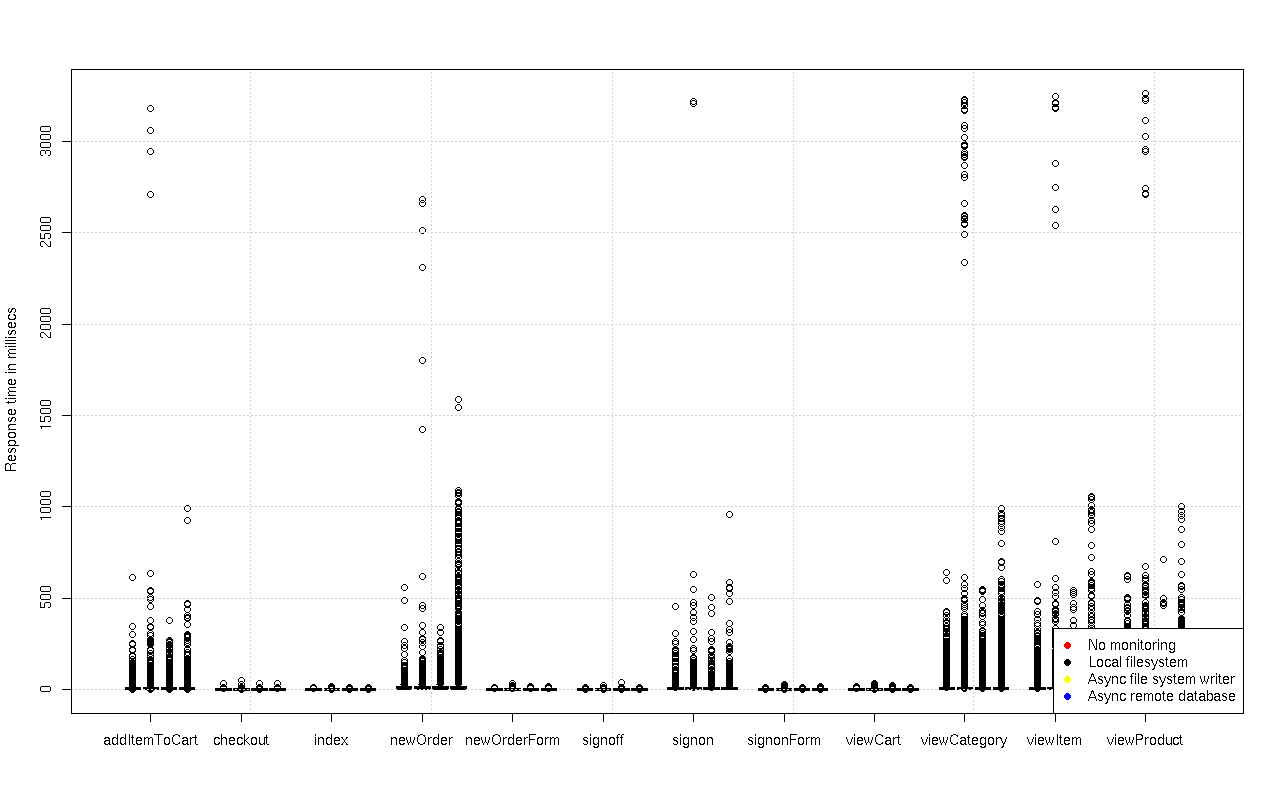
\includegraphics[width=\textwidth]{MonitoringOverhead1.png}
%  % MonitoringOverhead2.png: 1280x800 pixel, 72dpi, 45.16x28.22 cm, bb=0 0 1280 800
%  \label{MonitoringOverhead1}
%  \caption{JPetStore: Comparison of Monitoring Overhead}
% \end{figure}


\begin{figure}
 \centering
 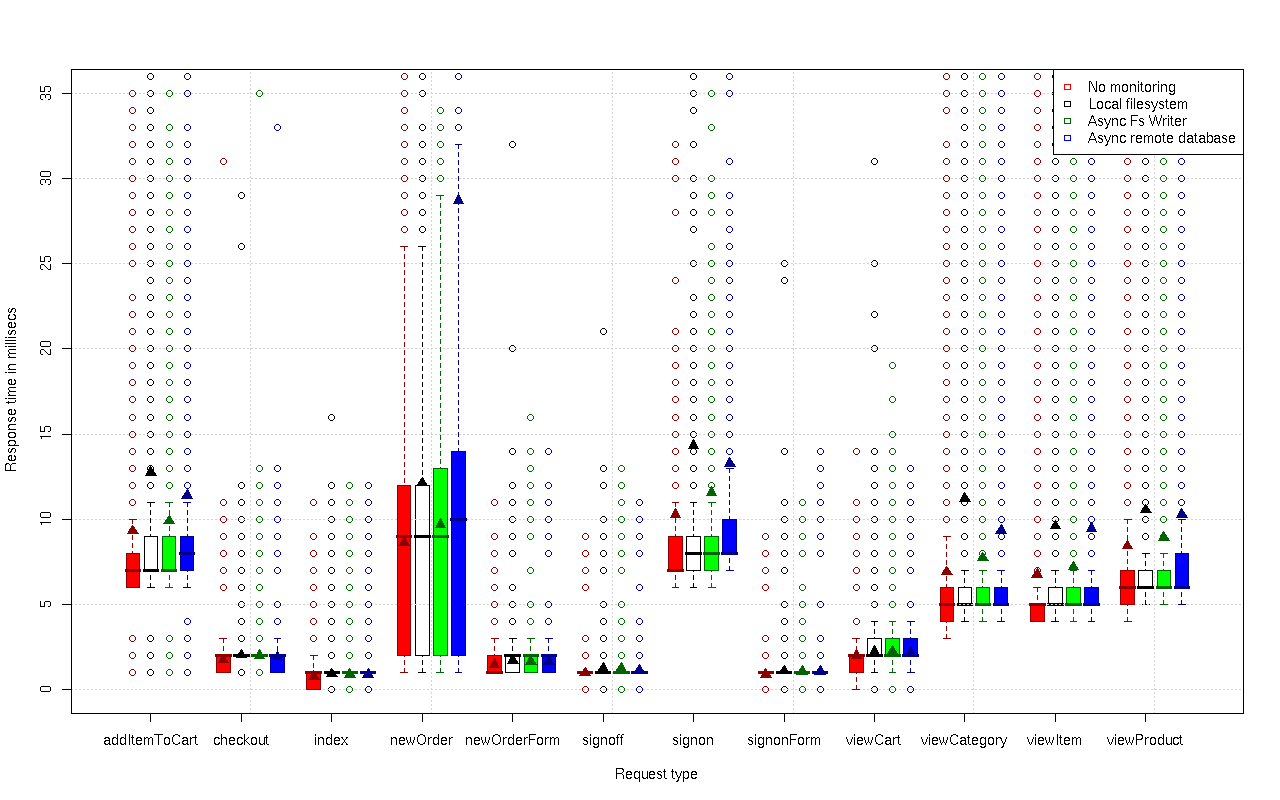
\includegraphics[width=\textwidth]{MonitoringOverhead2.png}
 % MonitoringOverhead2.png: 1280x800 pixel, 72dpi, 45.16x28.22 cm, bb=0 0 1280 800
 \label{MonitoringOverhead2}
 \caption{JPetStore: Comparison of Monitoring Overhead. Triangles indicate the corresponding arithmetic mean.}
\end{figure}


\begin{table}
\centering
\begin{tabular}{rrrrr}
  \hline
 & TpmonFs & TpmonAsyncFS & TpmonAsyncDB & TpmonSyncDB \\
  \hline
addItemToCart & 0.37 & 0.06 & 0.22 & 4.99 \\
  checkout & 0.17 & 0.16 & 0.11 & 24.12 \\
  index & 0.22 & 0.19 & 0.16 & 43.51 \\
  newOrder & 0.41 & 0.13 & 2.34 & 4.99 \\
  newOrderForm & 0.17 & 0.12 & 0.11 & 23.83 \\
  signoff & 0.25 & 0.25 & 0.17 & 41.55 \\
  signon & 0.39 & 0.12 & 0.29 & 5.02 \\
  signonForm & 0.24 & 0.19 & 0.19 & 42.57 \\
  viewCart & 0.12 & 0.12 & 0.09 & 17.71 \\
  viewCategory & 0.63 & 0.12 & 0.35 & 6.91 \\
  viewItem & 0.42 & 0.06 & 0.40 & 6.72 \\
  viewProduct & 0.25 & 0.06 & 0.22 & 5.24 \\
   \hline
\end{tabular}
\caption{JPetStore: Relative average slowdown compared to no monitoring}\label{generatedTpmonPerfTabel}
\end{table}

\begin{table}
\centering
\begin{tabular}{rrrrr}
  \hline
 & TpmonFs & TpmonAsyncFS & TpmonAsyncDB & TpmonSyncDB \\
  \hline
addItemToCart & 3.42 & 0.59 & 2.09 & 46.36 \\
  checkout & 0.29 & 0.28 & 0.19 & 41.26 \\
  index & 0.16 & 0.14 & 0.12 & 32.02 \\
  newOrder & 3.53 & 1.08 & 20.11 & 42.78 \\
  newOrderForm & 0.24 & 0.18 & 0.16 & 34.37 \\
  signoff & 0.24 & 0.24 & 0.17 & 39.92 \\
  signon & 4.04 & 1.26 & 2.97 & 51.63 \\
  signonForm & 0.21 & 0.16 & 0.17 & 37.01 \\
  viewCart & 0.23 & 0.25 & 0.18 & 35.23 \\
  viewCategory & 4.31 & 0.84 & 2.43 & 47.53 \\
  viewItem & 2.84 & 0.44 & 2.68 & 45.32 \\
  viewProduct & 2.11 & 0.49 & 1.85 & 44.07 \\
   \hline
\end{tabular}\caption{JPetStore: Absolute average slowdown compared to no monitoring in milliseconds}\label{generatedTpmonPerfTabel2}
\end{table}




\subsection{Troubleshooting -- Why does \tpmon\ fail?}
\paragraph{\tpmon\ does not compile -- ``ant build'' fails} There can be several reasons why it fails. First you should ensure that
\tpmon's basic requirements (at least Java SD 5 (version number 1.5), and Apache Ant 1.7) are satisfied. Possible reasons for compilation failures are 
\begin{itemize}
 \item Your user account might use a Java version older than version number 1.5. Ensure that ``\texttt{java -version}'' reports at least 1.5.*  = version 5. 
\item Apache Ant might use a Java version older than version number 1.5 or an old version of Ant is used. Ensure that ``\texttt{ant -v build}'' starts like this: \begin{lstlisting}[]
Apache Ant version 1.7.0 compiled on March 11 2007
Buildfile: build.xml
Detected Java version: 1.6 in: /opt/sun-jdk-1.6.0.02/jre
\end{lstlisting}
\end{itemize}

If an old Java version is used compilation will fail for Java Annotations (@ ... ) and generics (e.g., \texttt{Vector$<$String$>$} ...).


\paragraph{Checking the data storage part of \tpmon}
If \tpmon\ compiles, but it does not store monitoring data, it is a good
starting point to first check the simple parts of \tpmon\. The most simple
part is the logic responsible for storing observed response times into
the file system or database. This might fail, because of wrong 
database connection parameters, or in case of file system storage, 
the output folder or writing permissions might be missing.

To test the storage part of tpmon go to the folder \texttt{\$KIEKERHOME} and run
\begin{lstlisting}[caption={Testing the storage functionality},label={lst3}]
ant tpmon-test-storage
\end{lstlisting}

The results depends of the properties \texttt{storeInDatabase, monitoringEnabled} and \texttt{asyncFsWriter} in \texttt{tpmon.properties}. For storing in to the file system folder \texttt{$\backslash$tmp} the output might be something like this:

\begin{lstlisting}[caption={Output example for storage test},label={lst4}]
 [java] Starting test by adding 10000 monitoring events
     [java]  The vmid is 0cfeed62999abb27:a8b0fa2:119c26cc798:-7fff hashcode -1033091175
     [java]  Virtual Machine start time 1210147718971
     [java] Sleeping for 8 seconds
     [java] 10000 more monitoring points
     [java] Calling system.exit(0)
     [java] Tpmon: TpmonShutdownHook notifies all workers to initiate shutdown
     [java] Tpmon: TpmonShutdownHook can terminate since all workers are finished
\end{lstlisting}

This should create 20,000 lines of fake monitoring data created in a file \texttt{tpmon-*.dat} in the system's default temporary folder (e.g., \texttt{/tmp/} or \verb=C:\Docum...\USER...\Temp=):
\begin{lstlisting}[caption={Example fake monitoring data produced by the storage test},label={lst5}]
0;0component0method;sessionid;requestid;123;123;-1;0;0
0;1component1method;sessionid;requestid;123;123;-1;1;1
0;2component2method;sessionid;requestid;123;123;-1;2;2
0;3component3method;sessionid;requestid;123;123;-1;3;3
0;4component4method;sessionid;requestid;123;123;-1;4;4
0;5component5method;sessionid;requestid;123;123;-1;5;5
...
\end{lstlisting}

The storage test should be successful before other \tpmon\ tests are executed. Possible reasons for failures are:
\begin{itemize}
\item Both storage modes:
\begin{itemize}
 \item The file \texttt{\$KIEKERHOME/dist/KiekerTpmonCTW.jar} is outdated or missing (it contains the tpmon.properties used during runtime). Create it: \\ ``\texttt{ant build-tpmon-ctw}''.
\item You did not call ``\texttt{ant tpmon-test-storage}'' from the folder \texttt{\$KIEKERHOME}
\end{itemize}
\item Monitoring data is stored in the file system:
\begin{itemize}
 \item The folder configured for storing data does not exist. Try using a different folder a the system's default temporary folder (see Section \ref{sec.tpmon.properties}, properties on file system storage (1.3.1)).
\item The current user has no permissions to create a file \texttt{tpmon*} in the folder specified.
\end{itemize}
\item Monitoring data is stored in a database:
\begin{itemize}
\item Wrong database connection properties specified in \texttt{tpmon.properties}
\item The database driver is not within the classpath during execution
\item The database does not accept connections form your host. In case of MySQL, ensure that
you can connect to the database using the command line command ``\texttt{mysql}''.
\item There is no table for storing the monitoring data in the database -- create it with the SQL statement in the file
\texttt{table-for-monitoring.sql}. 
\item The file \texttt{\$KIEKERHOME/dist/KiekerTpmonCTW.jar} is outdated -- rebuild it with ``\texttt{ant build-tpmon-ctw}''.
\end{itemize}
\end{itemize}

\paragraph{Problem diagnosis using \textit{jconsole}}
\tpmon\ fails to monitor if essential libraries are not available during runtime. In all instrumentation variants, a \tpmon\ library must be present in the classpath (or found by the application server). A common load-time instrumentation problem is that the \aspectjweaverjar\ is not loaded as javaagent. 

The \textit{console} command-line tool, which is part of Sun's JDK, allows to diagnose these problems, as it shows which libraries are in the classpath and which javaagents have been added. If \textit{jconsole} is stared after the application to be monitored, it should offer to connect to the active Virtual Machine instances (see Figure~\ref{jconsolestartup}). As shown in Figure~\ref{jconsole}, \textit{jconsole} allows to check whether the \tpmon\ library is in the classpath and whether the \aspectjweaverjar\ is used as javaagent (which is required for AspectJ load-time instrumentation). Some older Java versions may require the additional Virtual Machine parameter \textit{-Dcom.sun.management.jmxremote} in order to use \textit{jconsole}.

\begin{figure}
 \centering
 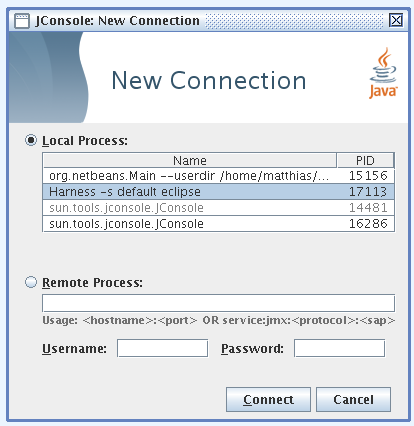
\includegraphics[width=7cm]{snapshot4b.png}
\caption{Attaching Java's \textit{console} to a Virtual Machine instance.}
 % snapshot4.png: 900x750 pixel, 72dpi, 31.75x26.46 cm, bb=0 0 900 750
 \label{jconsolestartup}
\end{figure}

\begin{figure}
 \centering
 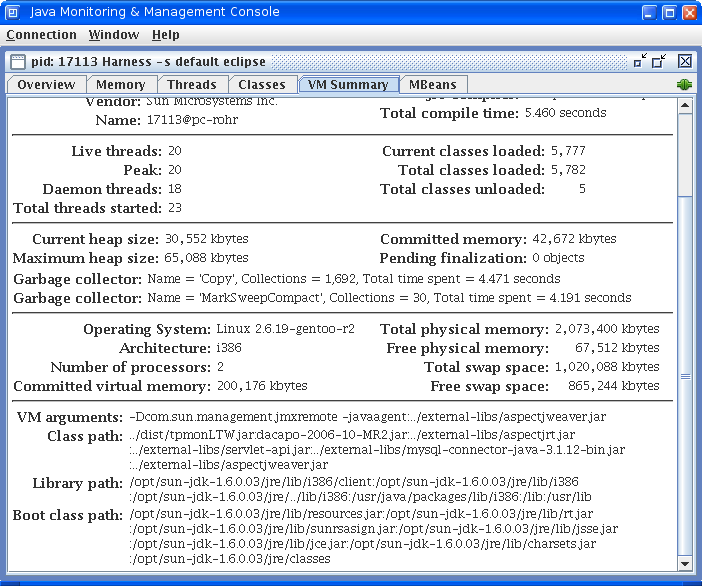
\includegraphics[width=12cm]{snapshot5.png}
 % snapshot4.png: 900x750 pixel, 72dpi, 31.75x26.46 cm, bb=0 0 900 750
 \caption{Problem diagnosis using \textit{jconsole}: A \tpmon\ library has to be within the classpath (except an application server is used that itself loads additional libraries). For load-time instrumentation, the \aspectjweaverjar\ has to be used as javaagent (see VM arguments).}\label{jconsole}
\end{figure}
% 
% 
% \section{\tpan\ quick start guide -- Hello world}\label{sec.tpan.tutorial}
% 
% ...
% 
% \section{\tpan: Kieker's Analysis and Visualization Component}\label{sec.tpan}
% 
% ... 


% 
% java -jar dacapo-2006-10-MR2.jar -converge eclipse default
% 

% 
% \section{Example: Instrumentation of the DaCapo Benchmark}
% As for each instrumentation, it is required to load \tpmonltw\ into the classpath and start the Java Virtual Machine with the \aspectjweaverjar\ as javaagent. Therefore, it is to expect that the DaCapo benchmark should be started like this:
% 
% \begin{lstlisting}[caption={Does not work: Instrumentation of DaCapo Benchmark (or other programs invoked using \texttt{java -jar})}],
% java -jar dacapo-2006-10-MR2.jar -converge eclipse default
% \end{lstlisting}



\bibliographystyle{abbrvnat} 
\bibliography{KiekerMonitoring.bib}


\end{document}
